\chapter{T对偶、D膜与规范理论}

\lectureoverview{T对偶最初表现为半径为(R)的圆上的闭弦与\(\alpha'/R\)上的闭弦之间的精确等价。动量与缠绕互换角色，世界面导数\(\partial_\tau Y\)与\(\partial_\sigma Y\)也互换角色，由\(G_{\mu 5}\)与\(B_{\mu 5}\)导出的时空矢量同样互换。当把同样的操作施加于开弦时，Neumann端点条件变为Dirichlet条件。端点因此必须位于一个动力学D膜上。被限制在一张膜上的开弦在低能下产生阿贝尔规范理论；连接一叠膜的弦带有两个端点标记，产生非阿贝尔规范理论。终止于D3膜上的D弦提供相应的磁单极子。}

\section{为什么要回到T对偶？}

我们已经遇到过T对偶，但回到它是有理由的。它是表明弦理论所包含的内容远多于微扰弦的线索之一。一旦理解了它对开弦的后果，它就引出了D膜；D膜反过来又成为构造和研究量子场论的一种方式。因此，本讲的目的不仅仅是重复“小圆等价于大圆”这一口号。我们将足够仔细地重建论证，以看清这一口号如何把新的物理对象强加进理论之中。

最简单的设定是环面紧致化。一维环面就是一个圆。二维环面可以用一个对边等同的平行四边形来表示，三维环面则可以用一个对面等同的平行六面体来表示。同样的构造可以继续到更高维。我们将只保留一个紧致空间坐标，称为\(Y\)，以及一个代表性的非紧致坐标，称为\(X\)。时间也存在，但不在板书中画出。

选择标准约定
\begin{equation}
  Y\sim Y+2\pi R,
  \label{eq:l10-circle-identification}
\end{equation}
于是\(R\)是半径，\(2\pi R\)是周长。本讲常把紧致尺度简称为\(r\)，并略去\(2\pi\)与\(\alpha'\)的因子。我们将在推导中保留这些常规因子，并在有用时显示本讲的单位。

在讨论的前半部分，弦是闭弦且是有向的。取向是画在弦上的一支内禀箭头。把所有箭头处处反向不会改变任何实验；重要的是两根弦的相对取向。在分裂与合并过程中，箭头必须连续地连接。这是带符号的守恒量将会出现的第一个迹象。

\begin{figure}[H]
  \centering
  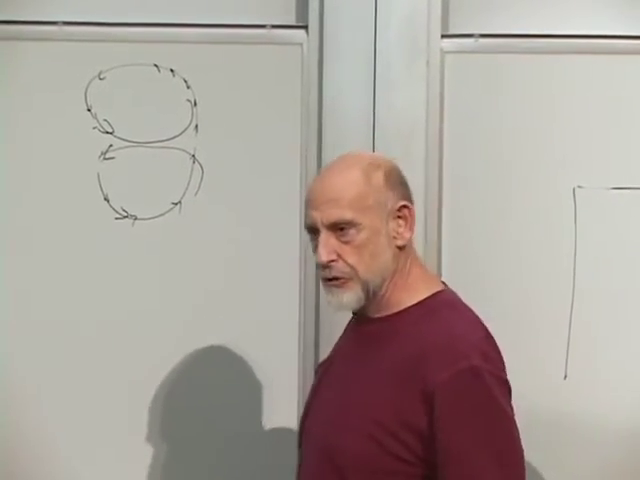
\includegraphics[width=0.72\textwidth]{lecture_10_figure_01.png}
  \caption{黑板上标出了两根闭弦及其相对取向。取向在分裂与合并过程中必须连续。}
  \lectureframe{00:05:40}
  \label{fig:l10-oriented-closed-strings}
\end{figure}

\begin{classroomqa}
\audiencequestion{如果世界面坐标从\(\sigma=0\)跑到\(2\pi\)，弦是否已经绕紧致方向走了一圈？\lecturetimestamp{00:08:42}}
\lecturerresponse{没有。坐标\(\sigma\)标记的是弦上的点；它并不标记紧致空间中的位置。每根闭弦都有一个周期性的参数\(\sigma\)，无论它是否缠绕。橡皮筋的类比很有用：即使橡皮筋没有绕在任何东西上，也可以给橡皮筋周围的分子编号。缠绕是映射\(Y(\tau,\sigma)\)的性质，而不是单由参数\(\sigma\)决定的性质。}
\end{classroomqa}

\begin{classroomqa}
\audiencequestion{紧致尺度是否也必须在大坐标\(X\)的每一个取值处都相同？\lecturetimestamp{00:10:00}}
\lecturerresponse{在一般的动力学紧致化中并非如此。我们从固定的圆开始，因为它是最干净的背景。后来，分量\(G_{55}\)将成为一个标量场，其取值度量第五方向的局部尺度，因此该尺度可以在普通时空上变化。}
\end{classroomqa}

\section{即使弦重新连接，缠绕也是守恒的}

一根未缠绕的弦可以穿过紧致方向而不绕它。缠绕的弦则不同：当\(\sigma\)绕闭弦走一圈时，嵌入\(Y(\tau,\sigma)\)前进一个或多个紧致圆的周期。因为弦是有向的，这一前进带有符号。弦可以沿正方向缠绕，也可以沿负方向缠绕。

守恒定律在合并的图像中最为清楚。取一根缠绕数为\(+1\)的弦和另一根缠绕数为\(-1\)的弦。它们相容的片段可以重新连接。所得位形具有零净缠绕数，并且可以形变为一根未缠绕的弦。黑板所描绘的正是这种相反取向的重新连接。

\begin{figure}[H]
  \centering
  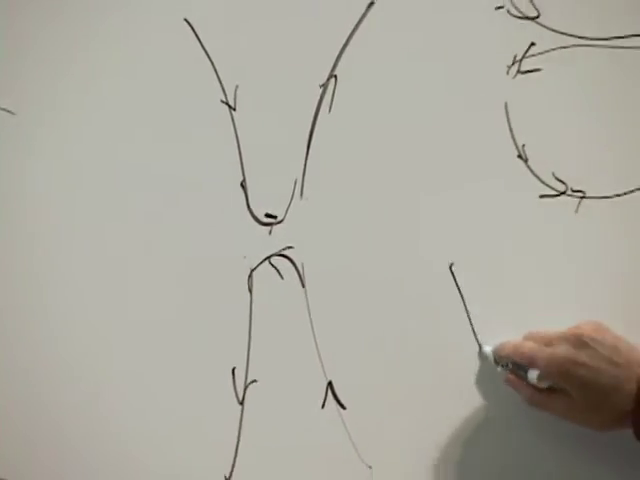
\includegraphics[width=0.72\textwidth]{lecture_10_figure_02.png}
  \medskip

  \begin{tikzpicture}[x=1cm,y=1cm,>=Latex]
    \draw[thick] (-4.0,0.3) circle (0.65);
    \draw[->,thick] (-4.55,0.58) arc (150:-145:0.65);
    \node at (-4.0,-0.65) {$w=+1$};
    \draw[thick] (-2.0,0.3) circle (0.65);
    \draw[<-,thick] (-2.55,0.58) arc (150:-145:0.65);
    \node at (-2.0,-0.65) {$w=-1$};
    \node at (-3.0,0.3) {$+$};
    \draw[->,thick] (-1.0,0.3) -- (0.3,0.3);
    \draw[thick] (1.4,0.3) ellipse (0.95 and 0.55);
    \node at (1.4,-0.65) {$w_{\rm total}=0$};
  \end{tikzpicture}
  \caption{相反绕数重新连接为零净绕数
  位形。下图是对黑板操作的清晰重构，而不是第二个动力学过程。}
  \lectureframe{00:13:20}
  \label{fig:l10-opposite-winding}
\end{figure}

现在用两根取向相同的弦重复该实验。它们可以连接，但不能退绕。结果携带任一根入射弦绕数的两倍。连接在一起的弦的数目改变了；总绕数没有改变。

\begin{figure}[H]
  \centering
  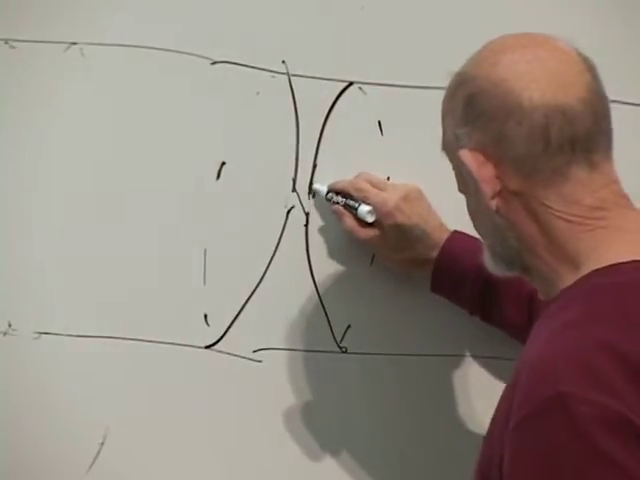
\includegraphics[width=0.72\textwidth]{lecture_10_figure_03.png}
  \medskip

  \begin{tikzpicture}[x=1cm,y=1cm,>=Latex]
    \draw[thick] (-4.0,0.3) circle (0.65);
    \draw[->,thick] (-4.55,0.58) arc (150:-145:0.65);
    \node at (-4.0,-0.65) {$w=+1$};
    \draw[thick] (-2.0,0.3) circle (0.65);
    \draw[->,thick] (-2.55,0.58) arc (150:-145:0.65);
    \node at (-2.0,-0.65) {$w=+1$};
    \node at (-3.0,0.3) {$+$};
    \draw[->,thick] (-1.0,0.3) -- (0.3,0.3);
    \draw[thick] (1.45,0.3) circle (0.78);
    \draw[thick] (1.45,0.3) circle (0.52);
    \draw[->,thick] (0.81,0.74) arc (145:-145:0.78);
    \node at (1.45,-0.78) {$w=+2$};
  \end{tikzpicture}
  \caption{同号绕数可以重新连接成一根双重缠绕的弦。
  连通性改变，而总绕数保持为二。}
  \lectureframe{00:16:40}
  \label{fig:l10-same-winding}
\end{figure}

这一区别在每一个允许的过程中都保持不变。总绕数一百可以由一根缠绕一百次的弦携带，由两根各缠绕五十次的弦携带，或由一百根单次缠绕的弦携带。弦可以在这些描述之间分裂和连接，但有符号之和保持为一百。我们将其记为\(w\in\mathbb Z\)。

\section{动量模式与绕数模式}

守恒本身还不是对偶性。接下来我们比较能量。一个绕紧致圆运动的态具有量子化动量
\begin{equation}
  p_Y=\frac{n}{R},
  \qquad n\in\mathbb Z.
  \label{eq:l10-compact-momentum}
\end{equation}
对于一个其他质量贡献可以忽略的态，紧致运动贡献\(E_{\rm mom}=|n|/R\)。正的和负的\(n\)表示相反的运动方向，而能量为正。

\begin{figure}[H]
  \centering
  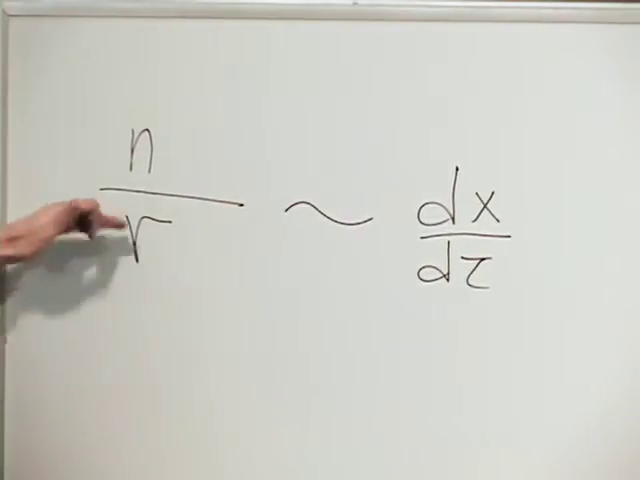
\includegraphics[width=0.72\textwidth]{lecture_10_figure_04.png}
  \caption{黑板上的紧致动量量子数。讲义将动量示意性地写为紧致速度的积分。}
  \lectureframe{00:21:30}
  \label{fig:l10-compact-momentum-board}
\end{figure}

一根缠绕\(|w|\)次的弦具有长度\(2\pi |w|R\)。以基本弦张力
\begin{equation}
  T_{\rm F}=\frac{1}{2\pi\alpha'},
\end{equation}
其绕数能量为
\begin{equation}
  E_{\rm wind}=T_{\rm F}(2\pi |w|R)
  =\frac{|w|R}{\alpha'}.
  \label{eq:l10-winding-energy}
\end{equation}
在讲义单位\(\alpha'=1\)下，这简单地就是\(E_{\rm wind}=|w|R\)。

当半径变化时，两座能级塔的行为相反。对于\(R\gg
\sqrt{\alpha'}\)，动量能级间距小，而绕数能级间距大。对于\(R\ll\sqrt{\alpha'}\)，动量能级间距大，而绕数能级间距小。

\begin{figure}[H]
  \centering
  \begin{minipage}[t]{0.48\textwidth}
    \centering
    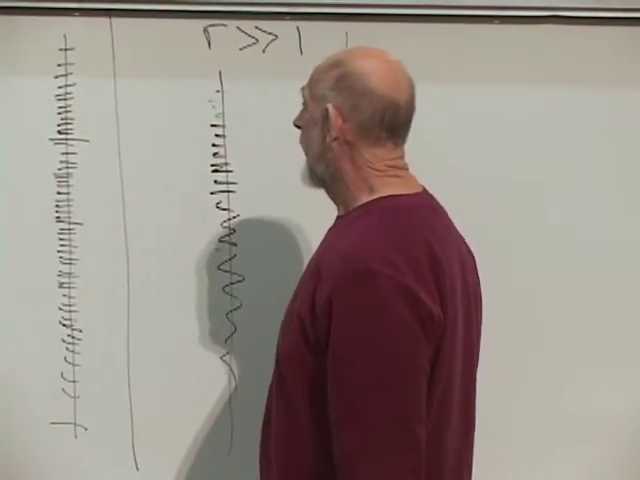
\includegraphics[width=\linewidth]{lecture_10_figure_05.png}
    \par\smallskip
    \textit{大紧致半径。}
  \end{minipage}\hfill
  \begin{minipage}[t]{0.48\textwidth}
    \centering
    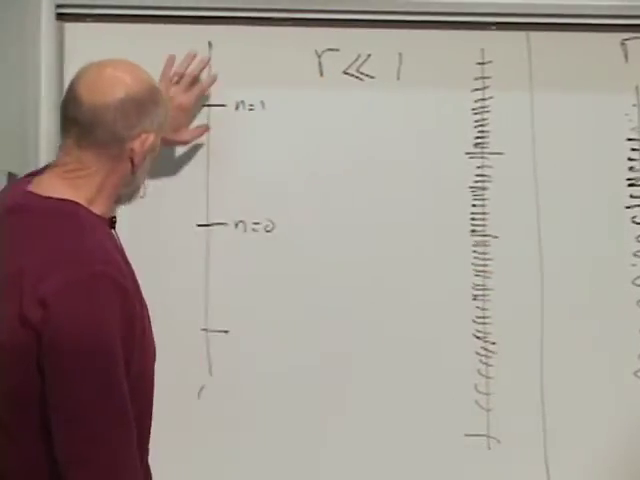
\includegraphics[width=\linewidth]{lecture_10_figure_06.png}
    \par\smallskip
    \textit{小紧致半径。}
  \end{minipage}
  \caption{黑板上的两个谱比较。当半径被反转时，稀疏和稠密的能级塔交换角色。}
  \lectureframe{00:25:30--00:26:00}
  \label{fig:l10-dual-spectra-board}
\end{figure}

清晰的示意图为
\begin{figure}[H]
  \centering
  \begin{adjustbox}{max width=\linewidth}
  \begin{tikzpicture}[x=1cm,y=0.74cm,>=Latex]
    \node[font=\bfseries] at (-3.6,6.2) {$R\gg\sqrt{\alpha'}$};
    \draw[->] (-5.1,0) -- (-5.1,5.5) node[above] {$E$};
    \foreach \y in {0.4,1.0,1.6,2.2,2.8,3.4,4.0,4.6}
      \draw (-5.35,\y)--(-4.85,\y);
    \node[align=center] at (-4.25,5.15) {momentum\\dense};
    \draw[->] (-2.2,0) -- (-2.2,5.5) node[above] {$E$};
    \foreach \y in {0.4,2.4,4.4}
      \draw (-2.45,\y)--(-1.95,\y);
    \node[align=center] at (-1.35,5.15) {winding\\sparse};

    \node[font=\bfseries] at (3.6,6.2) {$R\ll\sqrt{\alpha'}$};
    \draw[->] (2.2,0) -- (2.2,5.5) node[above] {$E$};
    \foreach \y in {0.4,2.4,4.4}
      \draw (1.95,\y)--(2.45,\y);
    \node[align=center] at (3.05,5.15) {momentum\\sparse};
    \draw[->] (5.1,0) -- (5.1,5.5) node[above] {$E$};
    \foreach \y in {0.4,1.0,1.6,2.2,2.8,3.4,4.0,4.6}
      \draw (4.85,\y)--(5.35,\y);
    \node[align=center] at (5.95,5.15) {winding\\dense};
  \end{tikzpicture}
  \end{adjustbox}
  \caption{能级间距论证的重构。当动量和绕数连同\(R\leftrightarrow\alpha'/R\)一起交换时，完整的弦谱不变。}
  \label{fig:l10-dual-spectra-redraw}
\end{figure}

假设一位观察者拿到这些谱中的一个，却没有被告知它是如何产生的。间距小的能级塔是大圆上的动量，还是小圆上的绕数？仅凭谱无法说明。弦理论给出更强的陈述：散射振幅也无法说明。这两种描述在
\begin{equation}
  n\longleftrightarrow w,
  \qquad
  R\longleftrightarrow \widetilde R=\frac{\alpha'}{R}.
  \label{eq:l10-radius-duality}
\end{equation}
下完全等价。不动点是
\begin{equation}
  R=\sqrt{\alpha'},
  \label{eq:l10-self-dual-radius}
\end{equation}
或在讲义单位下为\(R=1\)。在该半径处，额外的态可以变为无质量，并且规范对称性得到增强。

\begin{classroomqa}
\audiencequestion{绕数仅仅是为了重写谱而采用的数学便利吗？\lecturetimestamp{00:27:33}}
\lecturerresponse{不是。绕数标记闭弦希尔伯特空间的真实扇区，而这些扇区参与相互作用。``对偶''一词意味着动量描述和绕数描述是同一物理的不同坐标，而不是说一个扇区是另一个扇区的可选助记。}
\end{classroomqa}

\begin{classroomqa}
\audiencequestion{是否存在一个被映射到自身的半径？
\lecturetimestamp{00:27:58}}
\lecturerresponse{存在。自对偶值为
\(R=\sqrt{\alpha'}\)，在黑板所用单位下为\(R=1\)。两座能级塔在那里相遇，并且谱具有增强的对称性。}
\end{classroomqa}

\section{对偶性的世界面形式}

谱论证具有启发性，但世界面使这种交换更加精确。在共形规范中，与\(Y\)共轭的动量正比于\(\partial_\tau Y\)。因此总紧致动量具有形式
\begin{equation}
  P_Y=\frac{1}{2\pi\alpha'}
      \int_0^{2\pi}d\sigma\,\partial_\tau Y.
  \label{eq:l10-worldsheet-momentum}
\end{equation}
绕数为
\begin{equation}
  w=\frac{1}{2\pi R}
      \int_0^{2\pi}d\sigma\,\partial_\sigma Y
   =\frac{Y(2\pi)-Y(0)}{2\pi R}.
  \label{eq:l10-worldsheet-winding}
\end{equation}

\begin{classroomqa}
\audiencequestion{为什么导数的积分在闭合弦周围不会消失？\lecturetimestamp{00:32:33}}
\lecturerresponse{因为\(Y\)是一个周期性的靶空间坐标，而不是\(\sigma\)圆上的单值实函数。世界面点\(\sigma=2\pi\)与\(\sigma=0\)相同，但嵌入到覆盖线上的提升会改变\(2\pi wR\)。\(\partial_\sigma Y\)的积分衡量的正是这一移动。}
\end{classroomqa}

\begin{figure}[H]
  \centering
  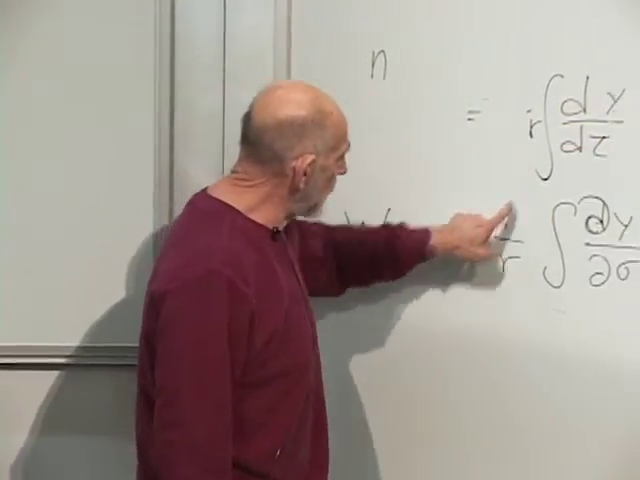
\includegraphics[width=0.76\textwidth]{lecture_10_figure_07.png}
  \caption{在板上完成两条线之后的动量与缠绕积分。常见的\(2\pi\)和\(\alpha'\)因子在讲座归一化中被省略。}
  \lectureframe{00:33:25}
  \label{fig:l10-momentum-winding-integrals}
\end{figure}

对于绕卷一次的弦，
\begin{equation}
  Y(\tau,\sigma+2\pi)=Y(\tau,\sigma)+2\pi R.
\end{equation}
对于缠绕数\(w\)，右侧的移动为\(2\pi wR\)。方程\eqref{eq:l10-worldsheet-winding}于是精确地计入了缠绕数。这就是板书简写\(w\sim R^{-1}\int
d\sigma\,\partial_\sigma Y\)的精确版本。

因此，T对偶的世界面表述为
\begin{equation}
  \partial_\tau Y\longleftrightarrow
  \partial_\sigma \widetilde Y,
  \qquad
  \partial_\sigma Y\longleftrightarrow
  \partial_\tau \widetilde Y,
  \label{eq:l10-derivative-duality}
\end{equation}
其中\(Y\)中的动量变为对偶坐标\(\widetilde Y\)中的缠绕，反之亦然。

\begin{classroomqa}
\audiencequestion{这是否意味着世界面坐标\(\tau\)和\(\sigma\)本身是相关的或互换的？\lecturetimestamp{00:34:39}}
\lecturerresponse{不。T对偶映射解，并交换紧致靶坐标的特定导数。它并不将世界面时间坐标与世界面空间坐标等同起来。}
\end{classroomqa}

\section{为什么缠绕态无法避免}

人们可能会问，当存在未缠绕态时，弦为什么还会处于缠绕态。弦并不按偏好选择自己的状态。碰撞中提供的能量会将它拉伸。一个能量足够高、高度畸变的弦可以重新连接成两根具有相反缠绕的弦。它们的总缠绕仍然为零，但在分裂之后，这两根弦可能分开。这对弦中的一个可以被送到很远的地方，使观察者面对一根看似孤立的缠绕弦。

\begin{figure}[H]
  \centering
  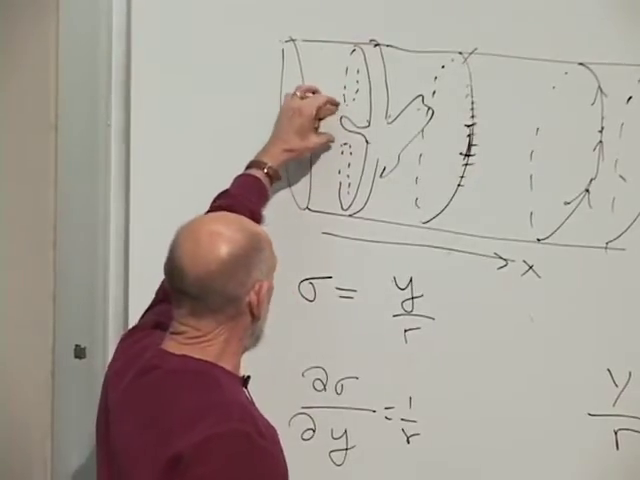
\includegraphics[width=0.76\textwidth]{lecture_10_figure_08.png}
  \caption{一个高度拉伸的零净缠绕构型，重新连接后相反缠绕的弦可以从中分离。}
  \lectureframe{00:36:15}
  \label{fig:l10-winding-pair-production}
\end{figure}

能量阈值由缠绕能设定。在一个大圆上，需要很大的碰撞能量才能将足够多的弦沿紧致方向拉伸。然而，在阈值以上，缠绕--反缠绕对产生不能被禁止。类比是光子碰撞产生电子--正电子对。总电荷仍然为零，但带电粒子确实存在并且可以被分开。缠绕守恒以同样的方式起作用。

这个类比不只是口头上的。紧致动量和缠绕表现为两个不同的荷量子数。在相应的约化描述中，同号相斥，异号相吸。因此，我们应当寻找传递这些力的两个矢量场。

\section{来自五维引力的动量荷}

从五维引力开始。令大写指标\(M,N\)遍历四个普通时空方向和紧致的第五方向。度规分解为
\begin{equation}
  G_{MN}\quad\longrightarrow\quad
  \bigl\{G_{\mu\nu},\,G_{\mu5},\,G_{55}\bigr\}.
  \label{eq:l10-metric-decomposition}
\end{equation}
对称分量\(G_{5\mu}\)除了\(G_{\mu5}\)之外不包含新信息。

\begin{figure}[H]
  \centering
  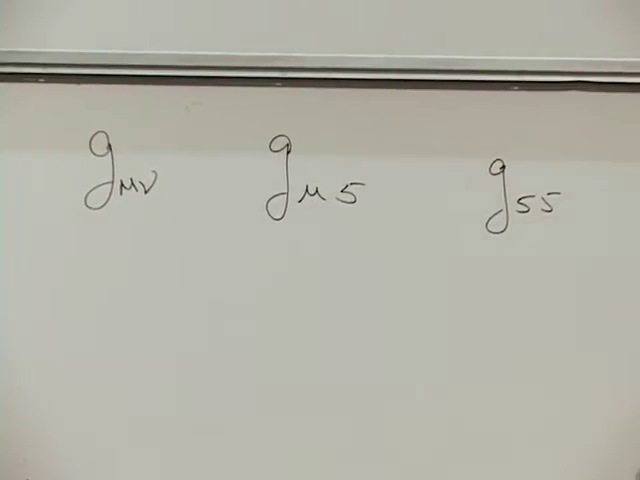
\includegraphics[width=0.74\textwidth]{lecture_10_figure_09.png}
  \caption{五维度规分量的独立分组：\(G_{\mu\nu}\)、\(G_{\mu5}\)和\(G_{55}\)。}
  \lectureframe{00:44:05}
  \label{fig:l10-metric-components}
\end{figure}

从四维观点看，
\begin{align}
  G_{\mu\nu} &\quad\hbox{is a spacetime metric},\\
  G_{\mu5} &\equiv A_\mu\quad\hbox{is a vector field},\\
  G_{55} &\equiv e^{2\varphi}\quad\hbox{is a scalar modulus}.
  \label{eq:l10-four-dimensional-fields}
\end{align}
标量\(\varphi\)衡量紧致方向的尺度。它可以在普通时空上平滑变化，因此\(\varphi\)的波就是第五维半径的波。

\begin{figure}[H]
  \centering
  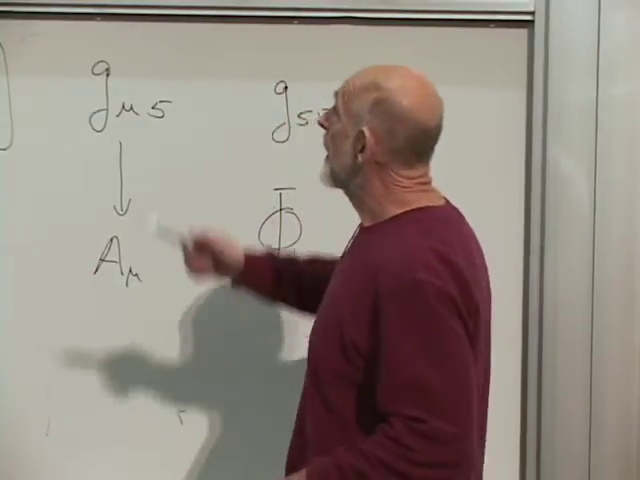
\includegraphics[width=0.74\textwidth]{lecture_10_figure_10.png}
  \caption{板书将\(G_{\mu5}\)等同于矢量\(A_\mu\)，将\(G_{55}\)等同于标量\(\Phi\)。}
  \lectureframe{00:47:40}
  \label{fig:l10-vector-and-radius-modulus}
\end{figure}

混合引力分量的源是混合动量流。特别地，沿第五方向的动量是\(G_{\mu5}\)的源。因此，四维观察者将整数\(n\)解释为耦合到\(A_\mu\)的电荷。这就是Kaluza--Klein机制：在高维几何中是动量的东西，在低维场论中变成电荷。

\editorialnote{讲座将来自\(G_{55}\)的标量粗略地称为``dilaton''。在这种约化中，它具体是半径模量。控制弦耦合的十维弦膨胀子是另一个场，尽管在改变标架和对偶下，低维标量组合可以混合。}

\begin{classroomqa}
\audiencequestion{标量\(\varphi\)是否正比于动量整数\(n\)？\lecturetimestamp{00:48:43}}
\lecturerresponse{不。整数\(n\)标记一个量子化态，并充当电荷。标量\(\varphi(x)\)是一个连续场，它决定局部的紧致化尺度。它可以随位置变化；它本身不是整数。}
\end{classroomqa}

\section{第二矢量场与缠绕荷}

缠绕也是类电荷的，但它不能以同样的方式耦合到同一个矢量。要看到第二个矢量，回到最初的闭弦激发。闭弦具有左行和右行振子模式。物理态满足能级匹配：左行和右行的总激发能级必须一致。

在玻色理论中，未激发态是快子。单个左行或右行振子会破坏能级匹配。因此第一个允许的无质量态包含每种振子各一个，
\begin{equation}
  \alpha_{-1}^{I}\widetilde\alpha_{-1}^{J}\ket{0;k}.
  \label{eq:l10-first-massless-state}
\end{equation}
指标\(I,J\)遍历横向空间方向，包括紧致方向。如果一个指标是普通的，另一个是\(5\)，则有两个类矢量振子态，
\begin{equation}
  \alpha_{-1}^{\mu}\widetilde\alpha_{-1}^{5}\ket{0;k},
  \qquad
  \alpha_{-1}^{5}\widetilde\alpha_{-1}^{\mu}\ket{0;k}.
  \label{eq:l10-two-vector-states}
\end{equation}

\begin{figure}[H]
  \centering
  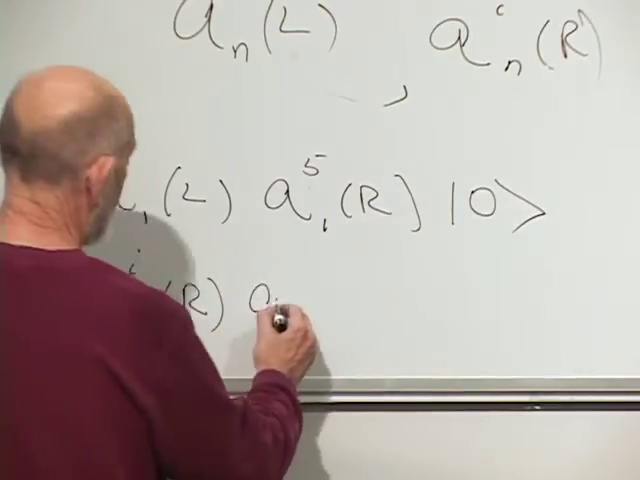
\includegraphics[width=0.76\textwidth]{lecture_10_figure_11.png}
  \caption{当其中一个极化沿紧致方向时，两种左--右振子排序成为四维矢量态。}
  \lectureframe{00:58:20}
  \label{fig:l10-two-vector-states-board}
\end{figure}

它们的对称和反对称组合属于不同的时空场：
\begin{align}
  \alpha_{-1}^{(\mu}\widetilde\alpha_{-1}^{5)}\ket{0;k}
    &\longleftrightarrow G_{\mu5},\\
  \alpha_{-1}^{[\mu}\widetilde\alpha_{-1}^{5]}\ket{0;k}
    &\longleftrightarrow B_{\mu5}.
  \label{eq:l10-g-and-b-vectors}
\end{align}
第一个是由紧致动量作为源的Kaluza--Klein矢量。第二个来自反对称的Kalb--Ramond场，并由弦缠绕作为源。因此，约化理论包含两个类光子场，每个电荷扇区各一个。

如果两个振子指标都沿紧致方向，则该态是与紧致化模量相关的标量。如果两者都在普通横向方向上，则对称无迹部分为引力子，反对称部分为\(B_{\mu\nu}\)，而迹则贡献到一个标量扇区。

\begin{classroomqa}
\audiencequestion{这些态中哪一个是单态，哪一个是三重态？\lecturetimestamp{01:00:21}}
\lecturerresponse{这种分类在这里不是有用的分类。两个混合态都作为四维矢量变换。它们的和与差将对称的度规极化与反对称的\(B\)场极化分开。具有两个紧致指标的态反而是四维标量。}
\end{classroomqa}

休息前得到的完整字典是
\begin{equation}
  \boxed{
  \begin{gathered}
    n\leftrightarrow w,
    \qquad
    R\leftrightarrow\dfrac{\alpha'}{R},\\
    \partial_\tau Y\leftrightarrow\partial_\sigma\widetilde Y,
    \qquad
    G_{\mu5}\leftrightarrow B_{\mu5}.
  \end{gathered}}
  \label{eq:l10-complete-t-duality-map}
\end{equation}

\begin{figure}[H]
  \centering
  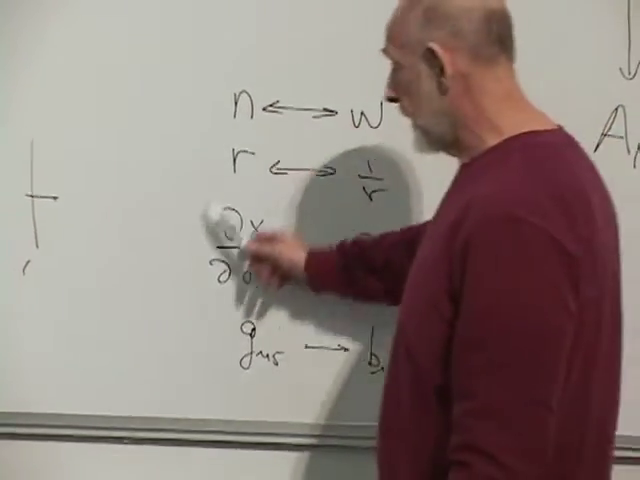
\includegraphics[width=0.72\textwidth]{lecture_10_figure_12.png}
  \caption{黑板上关于T对偶映射的总结：动量与缠绕、半径与倒数半径、世界面导数以及两个矢量场都被交换。讲演者部分遮挡了最后一行，因此该行在方程
  \eqref{eq:l10-complete-t-duality-map}中明确给出。}
  \lectureframe{01:02:20}
  \label{fig:l10-t-duality-map-board}
\end{figure}

不应将这一构造与如下主张混淆：刚刚列出的每个场都已经在观测到的粒子谱中被识别出来。在这一点上，它是紧致化弦理论的数学结果。有许多提议将这类结构与现象学联系起来，但这不是本讲所要解决的问题。

\section{开弦改变了问题}

休息之后，我们再次从开弦开始。闭弦可以具有稳定的缠绕，因为它没有端点可供缠绕滑脱。开弦有端点，因此没有类似的拓扑保护缠绕数。然而，T对偶是理论的精确对称性。这个对称性对开弦做了什么？

对于自由运动的端点，弦作用量的变分给出Neumann边界条件。在简单的\((X,Y)\)几何中，
\begin{equation}
  \left.\partial_\sigma X\right|_{\partial\Sigma}=0,
  \qquad
  \left.\partial_\sigma Y\right|_{\partial\Sigma}=0.
  \label{eq:l10-neumann-boundary}
\end{equation}
力学图像很直接。把弦看作由越来越小的质量元组成的链。对最后一个质量元施加非零的切向力，会使其加速度在其质量趋于零时发散。因此，自由端点会自行调整，直到端点净张力消失。人们也可以改为固定端点并提供所需的力，但那样端点就不再自由了。

\begin{figure}[H]
  \centering
  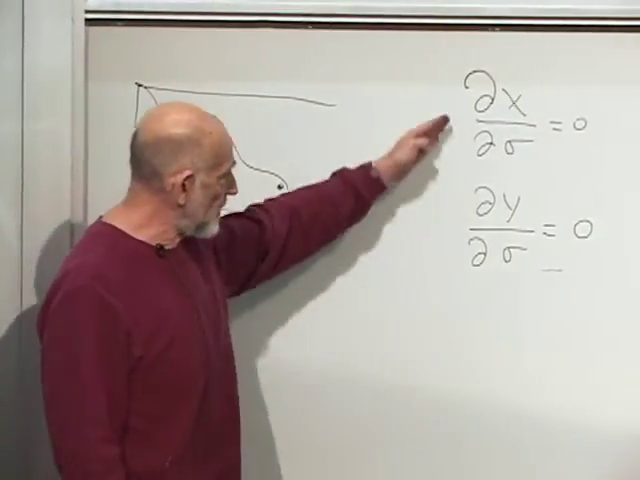
\includegraphics[width=0.76\textwidth]{lecture_10_figure_13.png}
  \caption{开弦及其完整的Neumann端点条件，\(\partial_\sigma X=\partial_\sigma Y=0\)。}
  \lectureframe{01:09:20}
  \label{fig:l10-neumann-board}
\end{figure}

现在只对紧致坐标\(Y\)做对偶化。非紧致坐标\(X\)保持不变。方程\eqref{eq:l10-derivative-duality}将第二个Neumann条件变为
\begin{equation}
  \left.\partial_\tau\widetilde Y\right|_{\partial\Sigma}=0.
  \label{eq:l10-dirichlet-time-derivative}
\end{equation}
因此，端点在対偶紧致方向上具有不依赖于时间的位置，
\begin{equation}
  \left.\widetilde Y\right|_{\partial\Sigma}=Y_0.
  \label{eq:l10-dirichlet-boundary}
\end{equation}
这就是Dirichlet边界条件。

\begin{figure}[H]
  \centering
  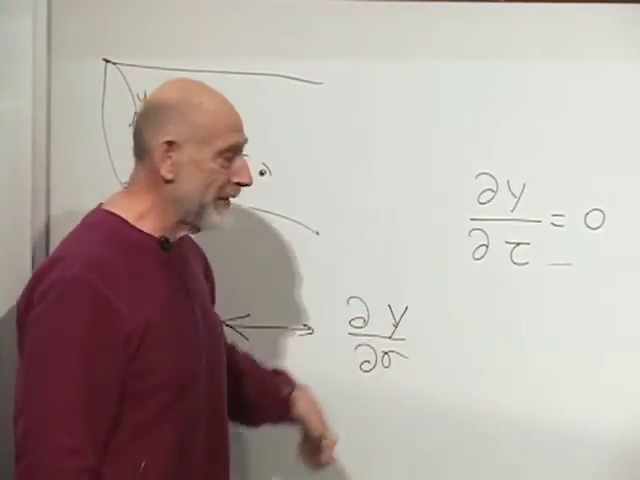
\includegraphics[width=0.76\textwidth]{lecture_10_figure_14.png}
  \medskip

  \begin{adjustbox}{max width=\linewidth}
  \begin{tikzpicture}[x=1cm,y=1cm,>=Latex]
    \node[align=center] at (-3.5,0.8)
      {Neumann\\\(\left.\partial_\sigma Y\right|_{\partial\Sigma}=0\)};
    \draw[->,thick] (-1.7,0.8) -- (1.3,0.8)
      node[midway,above] {$T_Y$};
    \node[align=center] at (3.4,0.8)
      {Dirichlet\\\(\left.\partial_\tau\widetilde Y\right|_{\partial\Sigma}=0\)};
    \node[align=center] at (3.4,-0.5)
      {\(\widetilde Y(\tau)=Y_0\) at each endpoint};
  \end{tikzpicture}
  \end{adjustbox}
  \caption{黑板上完成的对偶端点条件及其清晰的逻辑重构。T对偶将紧致方向上的自由度变为对偶方向上的固定端点位置。}
  \lectureframe{01:12:35}
  \label{fig:l10-neumann-to-dirichlet}
\end{figure}

\begin{classroomqa}
\audiencequestion{为什么対偶条件意味着端点是固定的？\lecturetimestamp{01:12:39}}
\lecturerresponse{因为\(\partial_\tau\widetilde Y=0\)在対偶化方向上的速度为零。无论端点在\(\widetilde Y\)中从哪里开始，它都停留在那里。其平行于未対偶化方向的坐标仍然是自由的。}
\end{classroomqa}

\section{持有端点的物体是D膜}

如果端点被固定，那么必须有某种东西能够把它保持在那里。因此，精确的T对偶要求存在一种新的物体，开弦可以终止于其上。这种物体就是D膜。字母\(D\)代表Dirichlet，而不是该物体的维度。在讲座的历史旁注中，这些物体或许会以Joseph Polchinski命名，因为他的分析使它们的动力学作用变得无可置疑，但已经确立的术语``p膜''使得Dirichlet成为自然的名称。

一个\(p\)膜具有\(p\)个空间维度。弦是一膜，膜是二膜，而延展的三维物体是三膜。一个D\(p\)膜是一个\(p\)膜，基本弦的端点在其横向方向上服从Dirichlet条件，而在与膜相切的方向上服从Neumann条件。

对偶论证中没有任何东西挑出\(Y_0\)的某一个值，因此D膜不可能是钉在宇宙中某个优先点上的刚性固定物。它必须是可移动的。相对论也禁止绝对刚性的延展物体，因此D膜可以涨落和弯曲。黑板上画出的简单平坦膜是它的平衡构型，而不是对其动力学的限制。

\begin{classroomqa}
\audiencequestion{开弦的两个端点是否必须具有相同的対偶坐标固定值？\lecturetimestamp{01:14:55}}
\lecturerresponse{一般来说不是。两个端点可以位于同一个D膜上，在这种情况下它们共享该膜的横向位置。它们也可以位于两个处于不同横向位置的不同D膜上，于是弦在它们之间拉伸。膜本身可以涨落和弯曲，因此端点轨迹不必保持为完全平坦的平面。}
\end{classroomqa}

\section{计算D膜的维度}

十维超弦理论有九个空间维度。假设T对偶在一个空间方向上施加Dirichlet条件。端点在其余八个方向上仍然是自由的，因此其允许的轨迹是一个八维D8膜。每增加一个独立的Dirichlet条件，就移除端点运动的一个方向。如果\(k\)个空间坐标被固定，那么
\begin{equation}
  p=9-k.
  \label{eq:l10-dp-counting}
\end{equation}

桌面给出了同一计数的三维版本。固定竖直坐标，指尖可以在二维桌面上移动。固定第二个坐标，它就只能沿一条线移动。固定全部三个坐标，它就被限制在一个点上。

\begin{figure}[H]
  \centering
  \begin{adjustbox}{max width=\linewidth}
  \begin{tikzpicture}[x=1.05cm,y=1cm,>=Latex]
    \draw[fill=blue!8] (-5.5,-0.7) -- (-2.5,-0.7) -- (-1.7,0.2)
      -- (-4.7,0.2) -- cycle;
    \node at (-3.6,-1.15) {one constraint: sheet};
    \draw[very thick,blue!60!black] (-0.9,-0.25) -- (1.3,-0.25);
    \node at (0.2,-1.15) {two constraints: line};
    \fill[blue!70!black] (4.1,-0.25) circle (0.09);
    \node at (4.1,-1.15) {three constraints: point};
    \draw[->] (-1.45,0.95) -- (-0.75,0.95);
    \draw[->] (2.25,0.95) -- (2.95,0.95);
    \node at (0.35,1.35) {each Dirichlet condition lowers \(p\) by one};
  \end{tikzpicture}
  \end{adjustbox}
  \caption{在桌面处使用的维度计数论证。D\(p\)膜是端点在其中仍可自由移动的轨迹。}
  \label{fig:l10-dp-counting-redraw}
\end{figure}

反复进行对偶化会生成D8膜、D7膜、D6膜等等，直到D0膜，它在空间中是点状的。如果没有空间方向被固定，一个D9膜填满全部九个空间维度，普通开弦可以在各处自由移动。讲座简要提到了D\((-1)\)膜；它们在欧几里得时空中是局域化的，其行为像瞬子，而不是像在时间中传播的普通粒子。

\editorialnote{维度阶梯是关于类型II理论合在一起的一个陈述。稳定的BPS D\(p\)膜在类型IIA中具有偶数\(p\)，在类型IIB中具有奇数\(p\)。沿一个圆进行T对偶会使\(p\)改变一，同时将类型IIA与类型IIB互换。}

\begin{classroomqa}
\audiencequestion{如果只有六个维度是紧致的，那么计数是否应当从六而不是从九开始减？\lecturetimestamp{01:20:49}}
\lecturerresponse{这一初等推导对紧致方向施行T对偶，但当一个圆变得任意小时，其对偶圆会变得任意大。在该极限下，它实际上是无限大的。因此，所得出的膜可以沿着在可及尺度上看似无限大的方向延展，也可以与之横截。维度\(p\)计数的是与膜相切的所有空间方向，而不仅仅是某一种推导中所用的紧致方向。}
\end{classroomqa}

D0膜是一种新型粒子。一根开弦可以从一个D0膜延伸到另一个D0膜，也可以回到同一个D膜，或者伸向一个非常遥远的膜。若把弦按字面意义延伸到空间无限远处，它便具有无限长度，因而具有无限能量，所以物理上有用的版本是把它的另一个端点放在另一个物体上。

下一个情形，即D1膜，本身是弦状的，但它并不是我们一开始所讨论的基本弦。它可以弯曲并闭合成自身，而基本弦可以终止于其上。它的张力对弦耦合常数的标度关系不同：
\begin{equation}
  T_{\rm D1}=\frac{1}{2\pi\alpha' g_s},
  \qquad
  T_{\rm F1}=\frac{1}{2\pi\alpha'}.
  \label{eq:l10-dstring-tension}
\end{equation}
在弱耦合\(g_s\ll1\)下，D弦比基本弦重得多，这解释了为什么它最初表现为一个质量巨大的锚点。

\begin{figure}[H]
  \centering
  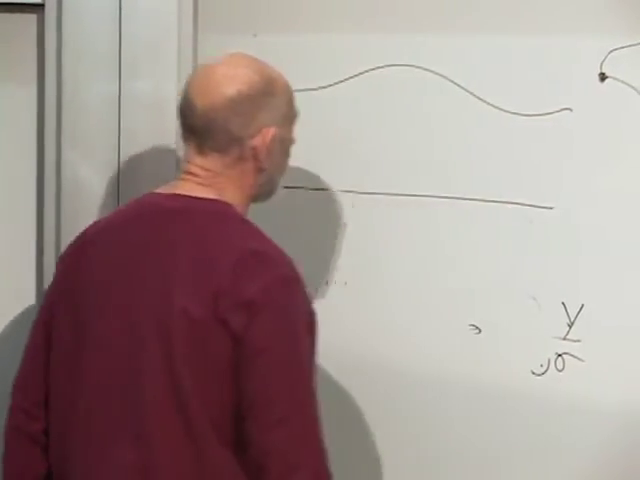
\includegraphics[width=0.76\textwidth]{lecture_10_figure_15.png}
  \caption{黑板上的D1膜：一个可弯曲的一维物体，不同于可以终止于其上的基本弦。}
  \lectureframe{01:24:20}
  \label{fig:l10-d1-brane}
\end{figure}

\begin{classroomqa}
\audiencequestion{T对偶是否既作用于弦，也作用于D膜？\lecturetimestamp{01:25:35}}
\lecturerresponse{是的。平行于D\(p\)膜的T对偶将其维度降低为D\((p-1)\)，而横截于它的T对偶将其维度升高为D\((p+1)\)。膜是对偶词典的一部分，而不是在对偶下保持不变的、外部的支撑物。}
\end{classroomqa}

\begin{classroomqa}
\audiencequestion{与膜相切的方向是否仍可以是紧致的？\lecturetimestamp{01:27:25}}
\lecturerresponse{是的。``相切''与``紧致''回答的是不同的问题。一个方向可以沿着膜，同时仍闭合成一个圆；它也可以是非紧致的。对端点而言，重要的是该方向上的边界条件是诺伊曼型还是狄利克雷型。}
\end{classroomqa}

D2膜是类似膜片的薄片。D3膜有三个空间维度。在真正高维的时空中，D3膜是一个三维子空间，而不是整个空间，尽管被限制在其上的观测者可能会把它体验为自己的整个空间世界。

\begin{figure}[H]
  \centering
  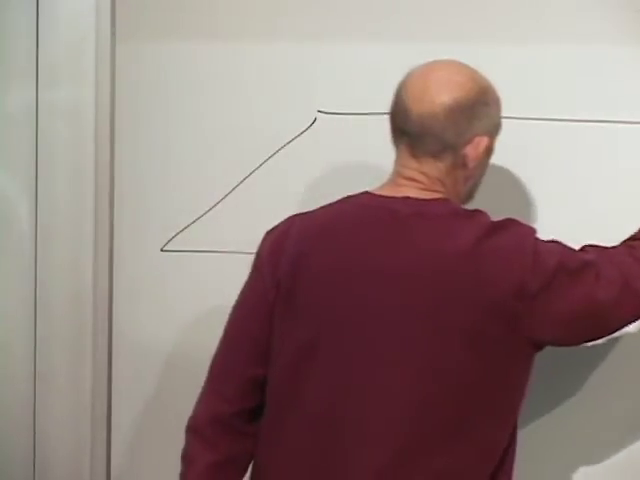
\includegraphics[width=0.76\textwidth]{lecture_10_figure_16.png}
  \caption{一个画成薄片的D2膜，弦的端点可以在其上移动。}
  \lectureframe{01:27:55}
  \label{fig:l10-d2-brane}
\end{figure}

这里给出的推导有意只是一个梗概。它本身并不能证明弦理论描述了自然。然而，在弦理论内部，一致性检验为数众多：对偶性、量子计算和数学结果都指向D膜是真正的动力学物体。

\section{开弦成为膜上的场}

取一个除此之外空无一物的D2膜，并把短开弦放在其上。每个端点都被限制在薄片内，因此整个低能激发沿着薄片运动。两根有向弦，若其相邻端点带有相容的箭头，便可以接合。接合后的弦之后可以再次分裂。若读作粒子历史，这些就是费曼图的顶点：两个粒子进入，一个中间激发传播，两个粒子出来。

\begin{figure}[H]
  \centering
  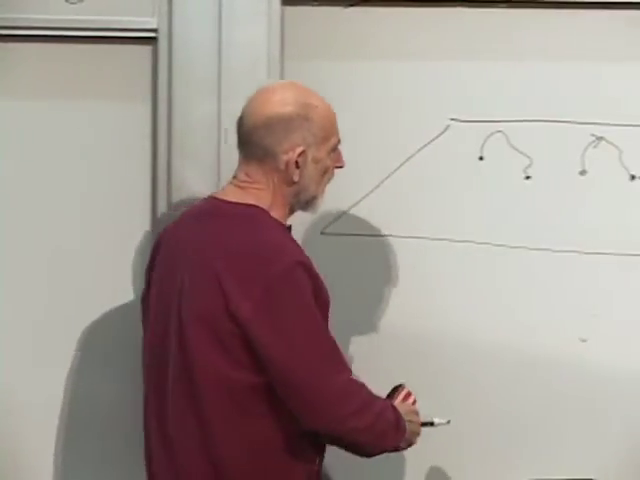
\includegraphics[width=0.76\textwidth]{lecture_10_figure_17.png}
  \caption{D2膜上的有向开弦通过相容的端点接合。在低能下，该过程被读作膜上的场论相互作用。}
  \lectureframe{01:29:55}
  \label{fig:l10-open-strings-on-brane}
\end{figure}

在远低于弦标度的能量下，内部振动谱塔不会被激发。剩下的无质量开弦态是膜世界体上的一个矢量场。对于单个膜，这是一个阿贝尔\(U(1)\)规范场，即电磁学在膜上的对应物。该场并不传播通过整个十维体空间；它的量子是开弦，其端点把它们保持在膜上。

\section{一叠膜产生非阿贝尔色}

现在把若干平行的膜放在彼此附近。对于三张膜，将它们标记为红、绿、蓝。一根有向弦具有一对有序的端点标签：它可以从红到绿、从绿到蓝、从红到红，等等。对于\(N\)张膜，无质量开弦态可以排列成一个\(N\times N\)矩阵
\begin{equation}
  A_\mu{}^{i}{}_{j},
  \qquad i,j=1,\ldots,N.
  \label{eq:l10-chan-paton-matrix}
\end{equation}
这些就是\(U(N)\)规范理论的Chan--Paton标签。

\begin{figure}[H]
  \centering
  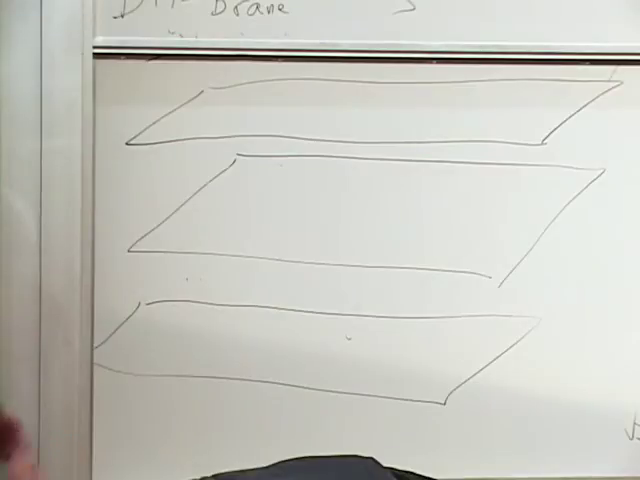
\includegraphics[width=0.76\textwidth]{lecture_10_figure_18.png}
  \medskip

  \begin{adjustbox}{max width=\linewidth}
  \begin{tikzpicture}[x=1cm,y=1cm,>=Latex]
    \draw[very thick,red!70!black] (-4.8,2.0)--(4.8,2.0);
    \draw[very thick,green!55!black] (-4.8,0.8)--(4.8,0.8);
    \draw[very thick,blue!70!black] (-4.8,-0.4)--(4.8,-0.4);
    \node[left] at (-4.8,2.0) {Red};
    \node[left] at (-4.8,0.8) {Green};
    \node[left] at (-4.8,-0.4) {Blue};
    \draw[->,thick] (-3.4,2.0) .. controls (-2.8,1.35) and (-2.3,1.15)
      .. (-1.7,0.8);
    \node at (-2.7,1.05) {$R\!G$};
    \draw[->,thick] (-0.6,0.8) .. controls (0.0,0.25) and (0.6,-0.05)
      .. (1.2,-0.4);
    \node at (0.1,0.0) {$G\!B$};
    \draw[->,thick] (2.1,2.0) .. controls (2.9,2.55) and (3.8,2.55)
      .. (4.3,2.0);
    \node at (3.2,2.65) {$R\!R$};
  \end{tikzpicture}
  \end{adjustbox}
  \caption{黑板上的三张平行膜，以及它们之间弦所携带的有序端点标签的清晰重构。}
  \lectureframe{01:33:15}
  \label{fig:l10-three-brane-stack}
\end{figure}

\begin{classroomqa}
\audiencequestion{一根弦真的能从红膜跑到绿膜，而不被其他图形挡住吗？\lecturetimestamp{01:35:07}}
\lecturerresponse{是的。这些膜嵌在更高维的空间中。二维的黑板图像只是一个投影，所以一根弦可以沿横向绕过另一条投影线。}
\end{classroomqa}

\begin{classroomqa}
\audiencequestion{一根红--绿弦必须与一根绿--蓝弦结合，才能变成红--蓝弦吗？\lecturetimestamp{01:35:39}}
\lecturerresponse{这就是基本的局部连接规则。相容的端点相遇，两段弦变成一根弦，其未连接的端点保留它们的红、蓝标签。更复杂的过程通过重复同一操作来构建。}
\end{classroomqa}

连接规则就是几何化的矩阵乘法。一根红--绿弦可以与一根绿--蓝弦连接，因为其中一根弦的绿端点与另一根弦的绿端点相容。结果是红--蓝弦：
\begin{equation}
  (R,G)\circ(G,B)\longrightarrow(R,B).
  \label{eq:l10-color-composition}
\end{equation}
重复的指标被连接并在内部消失。这与Yang--Mills相互作用顶点处出现的指标结构相同。

\begin{figure}[H]
  \centering
  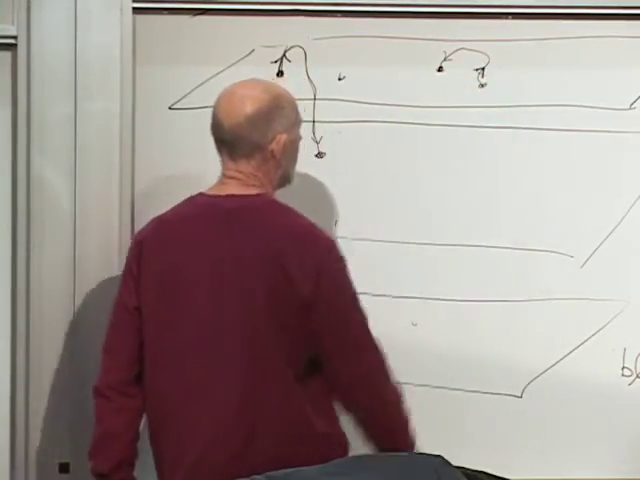
\includegraphics[width=0.76\textwidth]{lecture_10_figure_19.png}
  \caption{在膜堆上连接开弦。端点取向强制采用与非阿贝尔规范场相同的有序指标合成。}
  \lectureframe{01:36:30}
  \label{fig:l10-color-joining-board}
\end{figure}

对于三张重合的膜，完整的开弦规范群是\(U(3)\)，有九个矢量态。其代数分解为
\begin{equation}
  \mathfrak u(3)=\mathfrak{su}(3)\oplus\mathfrak u(1).
  \label{eq:l10-u3-decomposition}
\end{equation}
八个无迹组合具有QCD胶子的色结构，而对角质心\(U(1)\)是一个单独的阿贝尔场。

\editorialnote{讲座将九种色对组合之一描述为能够脱离并消失，从而留下八个胶子。精确的D膜陈述是：三张重合膜的堆给出\(U(3)\)，而不仅仅是\(SU(3)\)。要得到QCD八重态，需要分离、投影掉或以其他方式解耦对角\(U(1)\)。讲座的图像正确地启发了有序色指标，但它并不是对QCD的完整推导。}

类夸克物质只携带一个色指标。在膜图像中，它由一根弦表示，弦的一个端点位于色膜堆上，另一个端点位于另一张不同的、遥远的膜上。相对于色膜堆，只有一个端点作为色标签可见。反转取向就得到反粒子。一根类夸克弦和一根类反夸克弦若端点相容，就可以连接并离开色膜堆；两根取向相同的类夸克弦不能以这种方式湮灭。

由此得到的低能理论一般是超对称Yang--Mills理论，其附加物质由膜及其相交决定。它们与QCD足够接近，可以阐明非阿贝尔动力学，但它们并不自动就是标准模型。只有一张膜时，同样的构造约化为\(U(1)\)理论：短的膜--膜弦是类光子的，而到达第二个扇区的有向弦扮演正、负电荷的角色。

\section{D弦以磁单极子为终点}

现在故事中有两种类弦物体。原本的基本弦，即F弦，在D3膜上携带电流。D1膜，即D弦，在弱耦合下重得多。D弦也可以终止于D3膜上。它的端点在世界体规范场下不带电荷；它带磁荷。从D3膜上的观察者来看，该端点是一个磁单极子。

\begin{figure}[H]
  \centering
  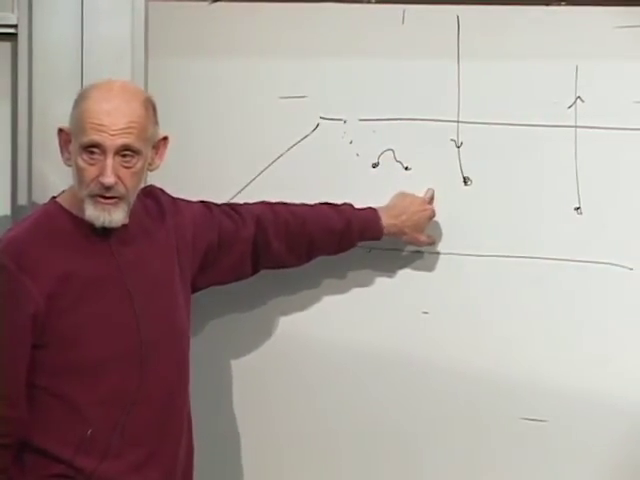
\includegraphics[width=0.76\textwidth]{lecture_10_figure_20.png}
  \medskip

  \begin{adjustbox}{max width=\linewidth}
  \begin{tikzpicture}[x=1cm,y=1cm,>=Latex]
    \draw[fill=blue!7] (-3.8,-0.5)--(2.6,-0.5)--(3.6,0.35)--(-2.8,0.35)--cycle;
    \node at (2.25,-0.95) {D3-brane};
    \draw[very thick,red!70!black] (0.0,3.0)--(0.0,0.0);
    \fill[black] (0.0,0.0) circle (0.08);
    \node[right] at (0.15,2.1) {D-string};
    \foreach \a in {25,65,115,155} {
      \draw[->,blue!65!black] (0.0,0.0)--({1.25*cos(\a)},{0.65*sin(\a)});
    }
    \node[align=center] at (4.8,1.7) {magnetic flux\\on the D3 worldvolume};
    \draw[->] (3.7,1.35)--(1.05,0.45);
  \end{tikzpicture}
  \end{adjustbox}
  \caption{黑板上的端点构造及其清晰解释。一根终止于D3膜上的D弦，对世界体规范理论而言表现为磁单极子。}
  \lectureframe{01:41:30}
  \label{fig:l10-dstring-monopole}
\end{figure}

质量等级结构也具有正确的定性形式。由于D弦张力带有因子\(1/g_s\)，在弱耦合下其端点比普通的电激发重得多。F弦与D弦端点之间的电/磁关系是IIB型弦理论更广泛对偶结构的一部分。

\begin{classroomqa}
\audiencequestion{D弦的端点是中性的吗？
\lecturetimestamp{01:42:19}}
\lecturerresponse{相对于基本弦端点所携带的电荷而言，它是中性的，但它并非不带电。它携带磁荷，因此是D3膜规范理论中的磁单极子。}
\end{classroomqa}

\section{该构造声称了什么，又没有声称什么}

从T对偶到膜的这条道路是历经数十年逐步拼合而成的，而非出自单一计算。一个最初为描述强子而提出的理论，变成了量子引力的候选理论。它的对偶性随后把D膜逼入谱中，而规范理论又作为终结于这些膜上的弦的低能动力学重新出现。在这个意义上，这门学科兜了一个完整的圈子。

D膜及相关的对偶构造已成为研究超对称规范理论、强耦合系统以及引力与场论之间联系的有力工具。它们还通过规范/引力对偶为流体和等离子体模型提供了启示。这一成功并不等同于直接推导出观测到的粒子谱。紧致化几何、膜位形、超对称破缺以及许多其他要素仍然有待选定。

\begin{classroomqa}
\audiencequestion{是什么决定了哪一个紧致维度被对偶化？
\lecturetimestamp{01:44:59}}
\lecturerresponse{从数学上说，只要所需对称性存在，就可以对任何紧致方向做对偶，并选择最方便的描述。从物理上说，在某一特定状态中实现的膜取向和紧致化数据，是由该状态的历史和动力学所选择的。}
\end{classroomqa}

\begin{classroomqa}
\audiencequestion{磁单极子构造由哪一种膜承载？
\lecturetimestamp{01:45:21}}
\lecturerresponse{规范理论所经历的世界是一张D3膜。D弦延伸到横向方向并终结于那张D3膜上；它的端点就是在该膜的三维空间中所见的磁单极子。}
\end{classroomqa}

\begin{classroomqa}
\audiencequestion{D弦也是有取向的吗？
\lecturetimestamp{01:45:55}}
\lecturerresponse{是的。反转D弦的取向会反转相应的荷。两种端点取向区分磁单极子与反磁单极子，正如取向对基本弦端点区分电荷一样。}
\end{classroomqa}

\begin{classroomqa}
\audiencequestion{这个简单的环面图像能解释手征粒子物理的左--右不对称性吗？
\lecturetimestamp{01:46:05}}
\lecturerresponse{仅凭它本身不能。平坦环面过于对称。手征谱需要更多结构，例如不对称的膜相交、orbifold投影，或在合适的Calabi--Yau几何上的紧致化。弦理论具有产生手征性的机制，但它们超出了这一初等T对偶构造的范围。}
\end{classroomqa}

我们追踪了一种对称性历经四种具体形式：谱的交换、世界面导数的交换、时空场的交换，最后是端点边界条件的交换。最后一种形式是决定性的。它把一种数学等价性转变为D膜的发现，并把开弦的动力学转变为其世界体积上的规范理论。到了这一步，用Susskind的话说，这场讲座已经用尽了它的时间、能量和动量。